\documentclass{article}
\usepackage{fancyvrb}
\usepackage{fancyhdr}
\usepackage{extramarks}
\usepackage{amsmath}
\usepackage{amsthm}
\usepackage{amsfonts}
\usepackage{tikz}
\usepackage{graphicx}
\usepackage{enumitem}
\usepackage[plain]{algorithm}
\usepackage{algpseudocode}
\usepackage[normalem]{ulem}
\usepackage{hyperref}
\usepackage{xcolor}
\usepackage{caption}
\usepackage{subcaption}
\usepackage{listings}% http://ctan.org/pkg/listings
\lstset{
  basicstyle=\ttfamily,
  mathescape
}

\usetikzlibrary{automata,positioning}

\topmargin=-0.45in
\evensidemargin=0in
\oddsidemargin=0in
\textwidth=6.5in
\textheight=9.0in
\headsep=0.25in

\linespread{1.1}

\pagestyle{fancy}
\lhead{\hmwkAuthorName}
\rhead{\hmwkClass\ (\hmwkClassInstructor): \hmwkTitle}
% \rhead{\firstxmark}
\lfoot{\lastxmark}
\cfoot{\thepage}

\renewcommand\headrulewidth{0.4pt}
\renewcommand\footrulewidth{0.4pt}

\setlength\parindent{0pt}

\newcommand{\hmwkTitle}{FP Progress Report}
\newcommand{\hmwkClass}{CSE 512}
\newcommand{\hmwkClassInstructor}{Jeffrey Heer}
\newcommand{\hmwkAuthorName}{Emily Gu | Ryan Drapeau | Vimala Jampala}

\date{}

\begin{document}

\begin{center}
\LARGE
\textbf{Final Project Progress Report}
\end{center}
\vspace{-15 pt}
\section*{Project Summary}

\vspace{-3 pt}
\begin{center}
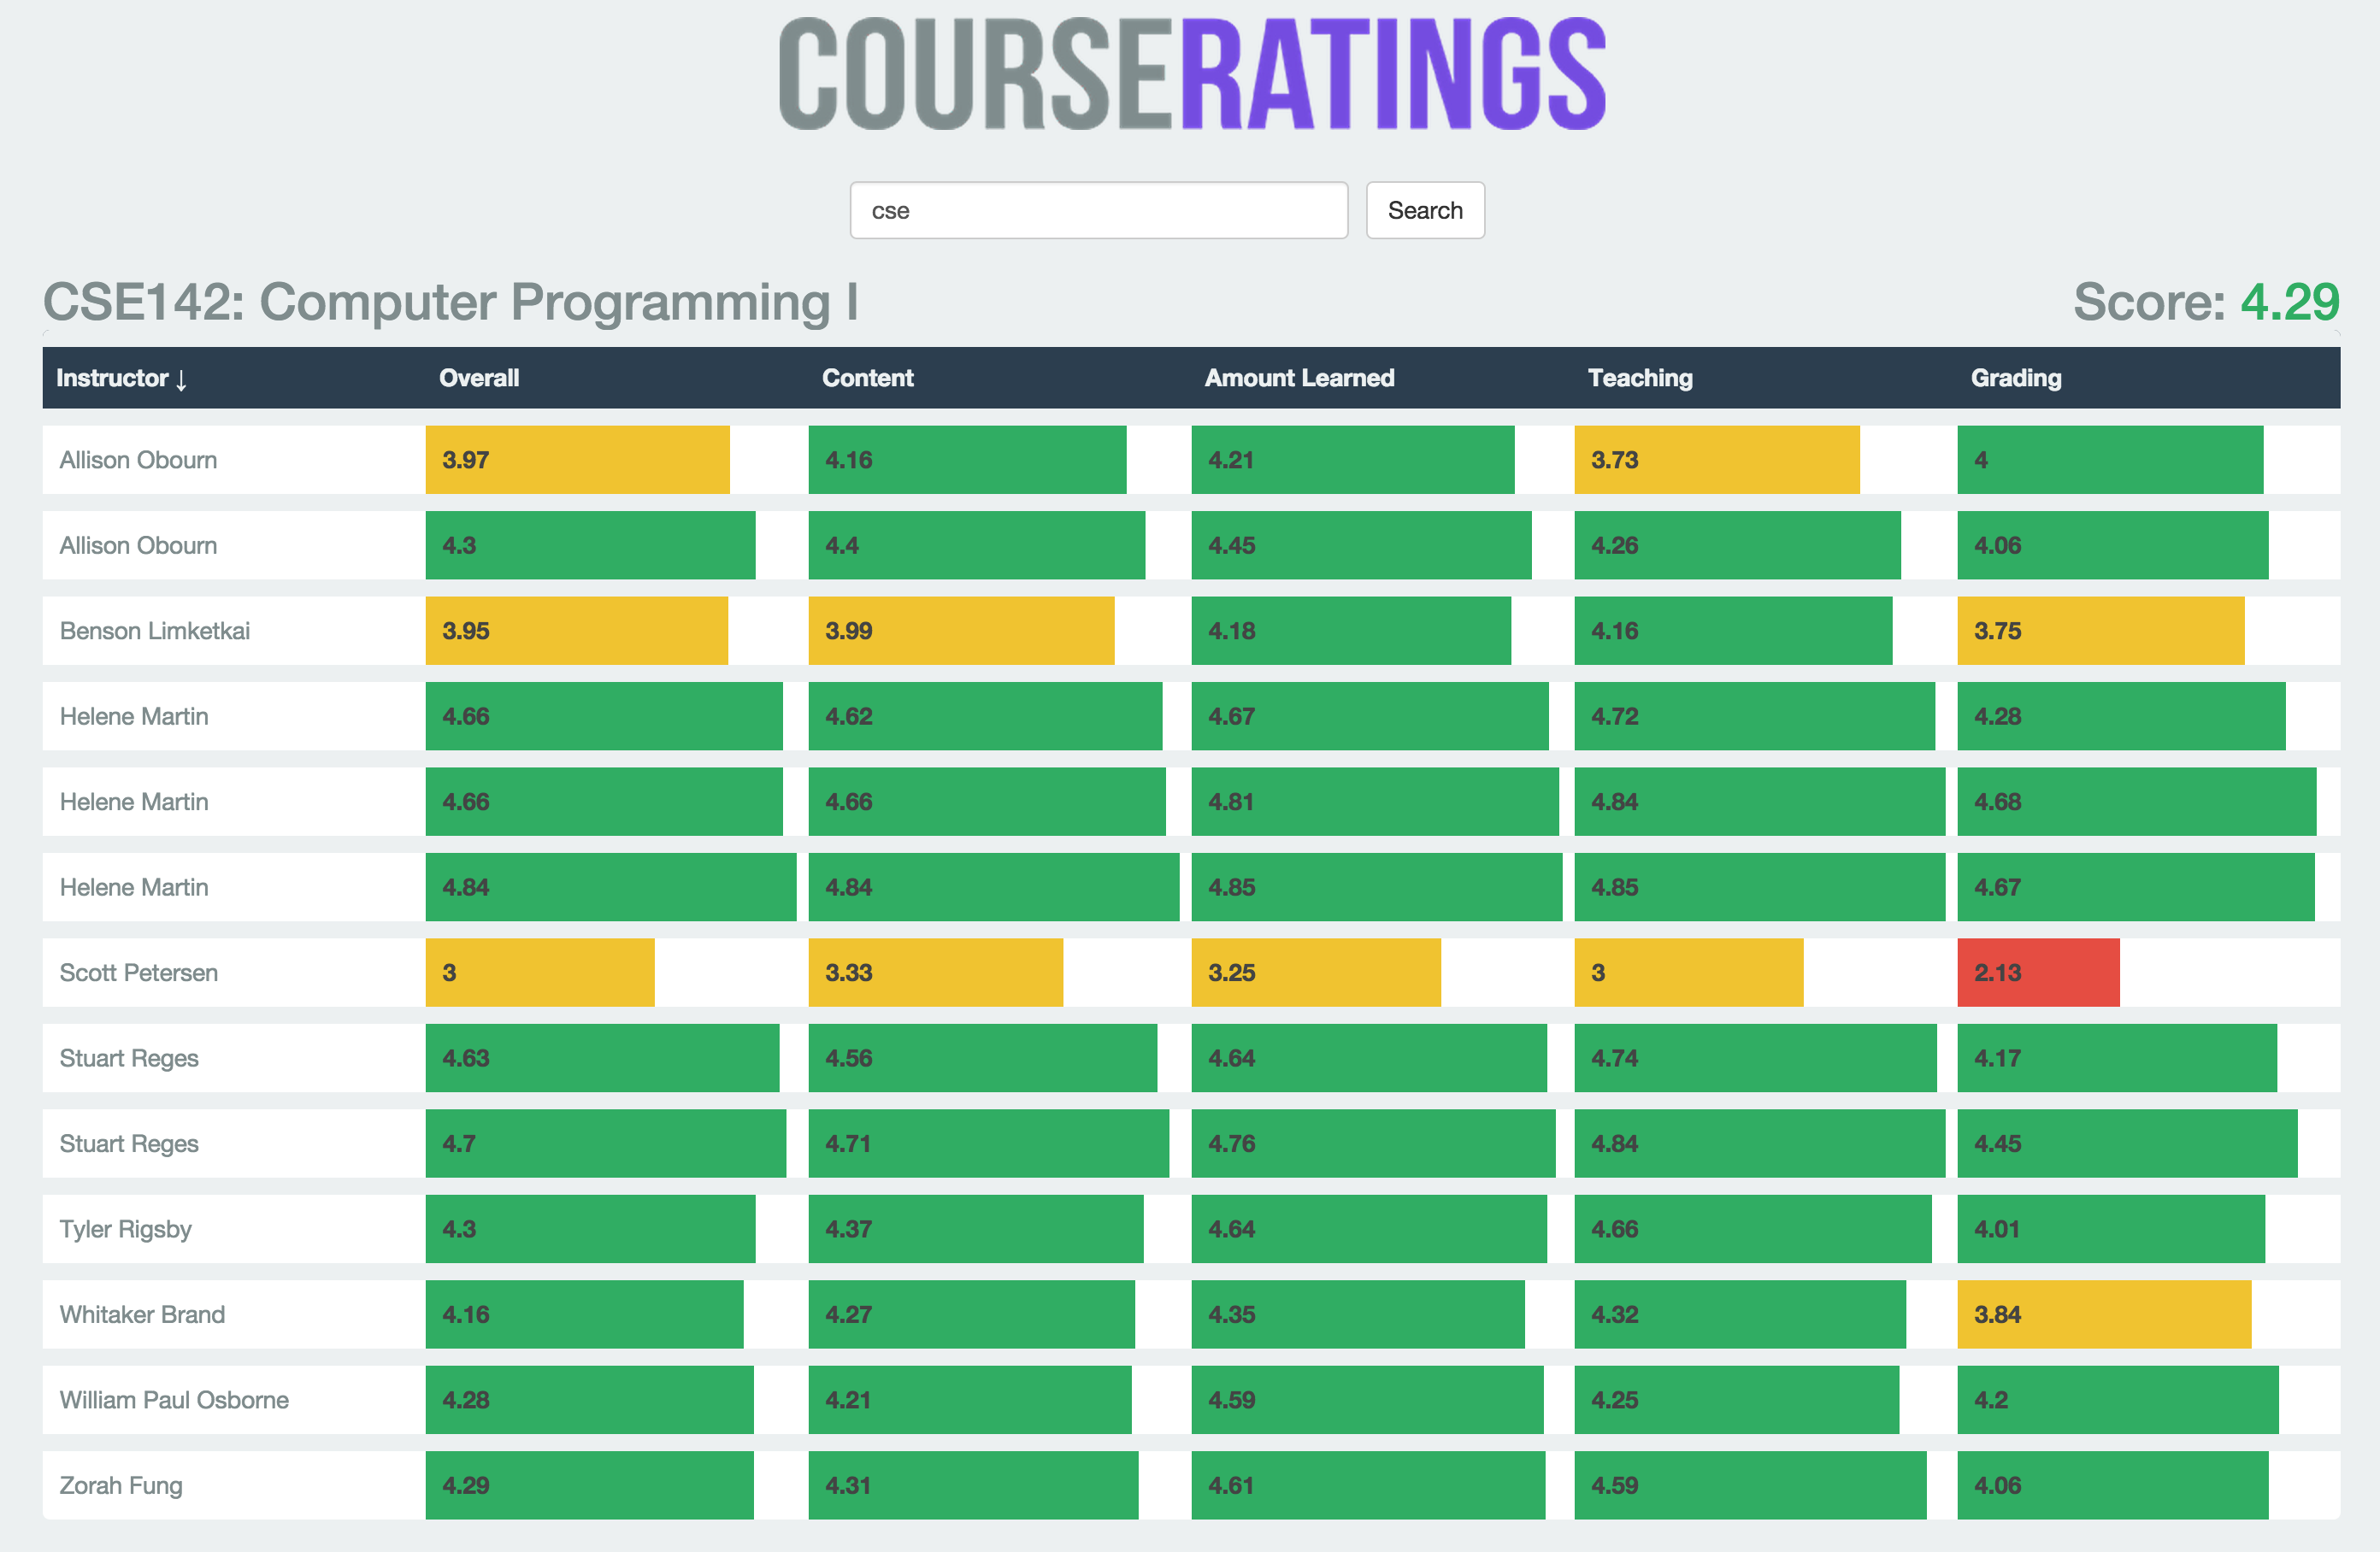
\includegraphics[width=0.7\textwidth]{cr.png}
\end{center}

We plan to continue development on our Assignment 3 project, CourseRatings, which visualizes the Course Evaluation Catalog in a more intuitive and user-friendly way. Currently, CourseRatings provides the option to search and sort through the vast amounts of data. The goal for this tool is to provide a way for students and instructors to find relevant and useful information for courses taught at the University of Washington. This will allow students to find good instructors and it will hold instructors responsible for providing an active and enjoyable learning environment in the classroom.
\vspace{-10 pt}
\section*{Literature Review}

\subsubsection*{UW Course Evaluation Catalog (CEC) \cite{cec}}
{\color{blue} \href{https://www.washington.edu/cec/toc.html}{https://www.washington.edu/cec/toc.html}}

\vspace{-3 pt}
\begin{center}
\begin{tabular}{ll}
    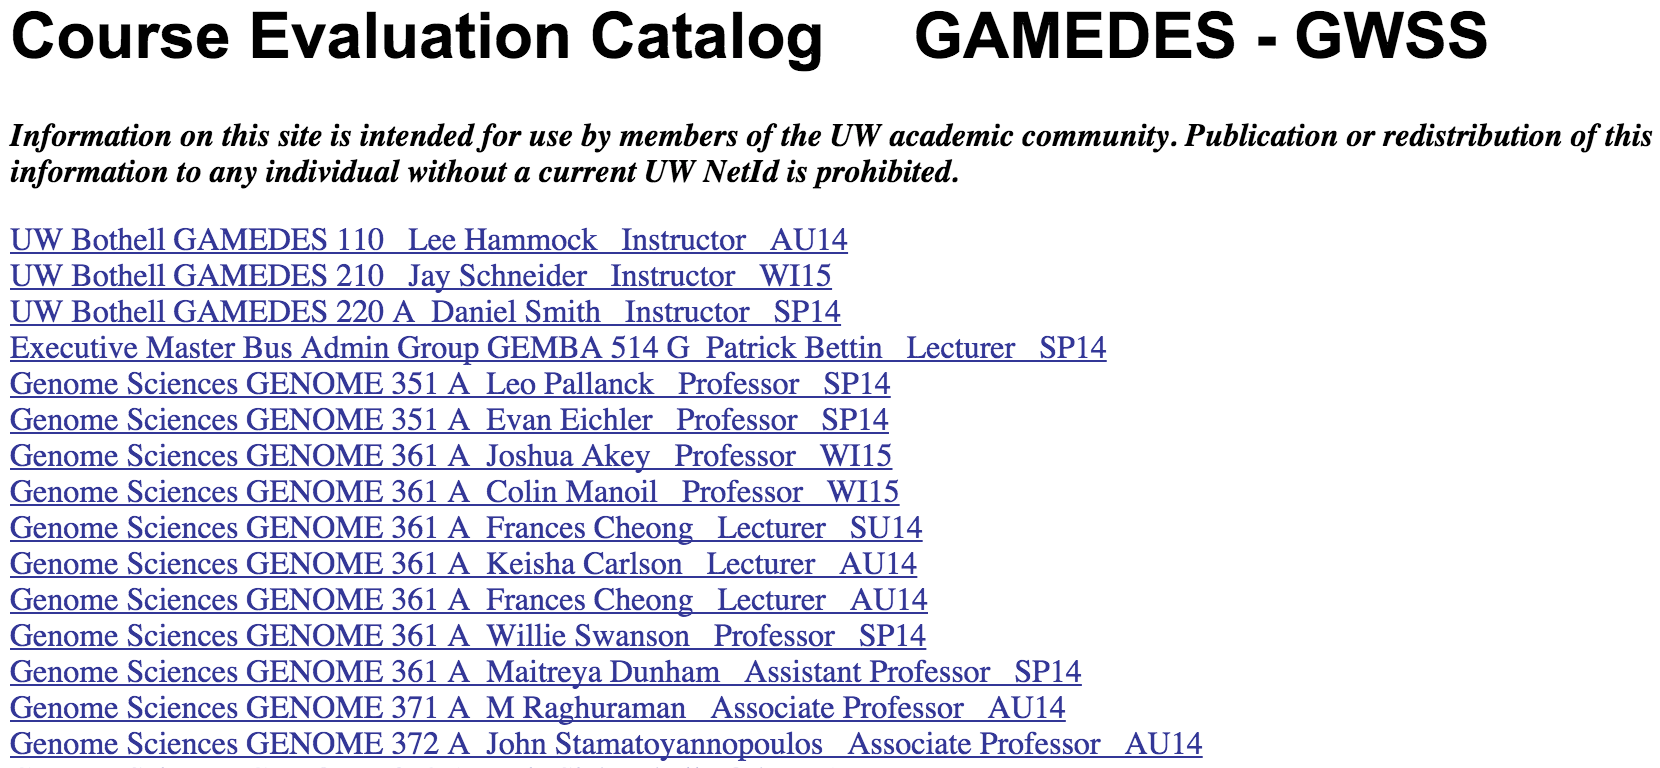
\includegraphics[width=0.54\textwidth]{cec.png}
    &
    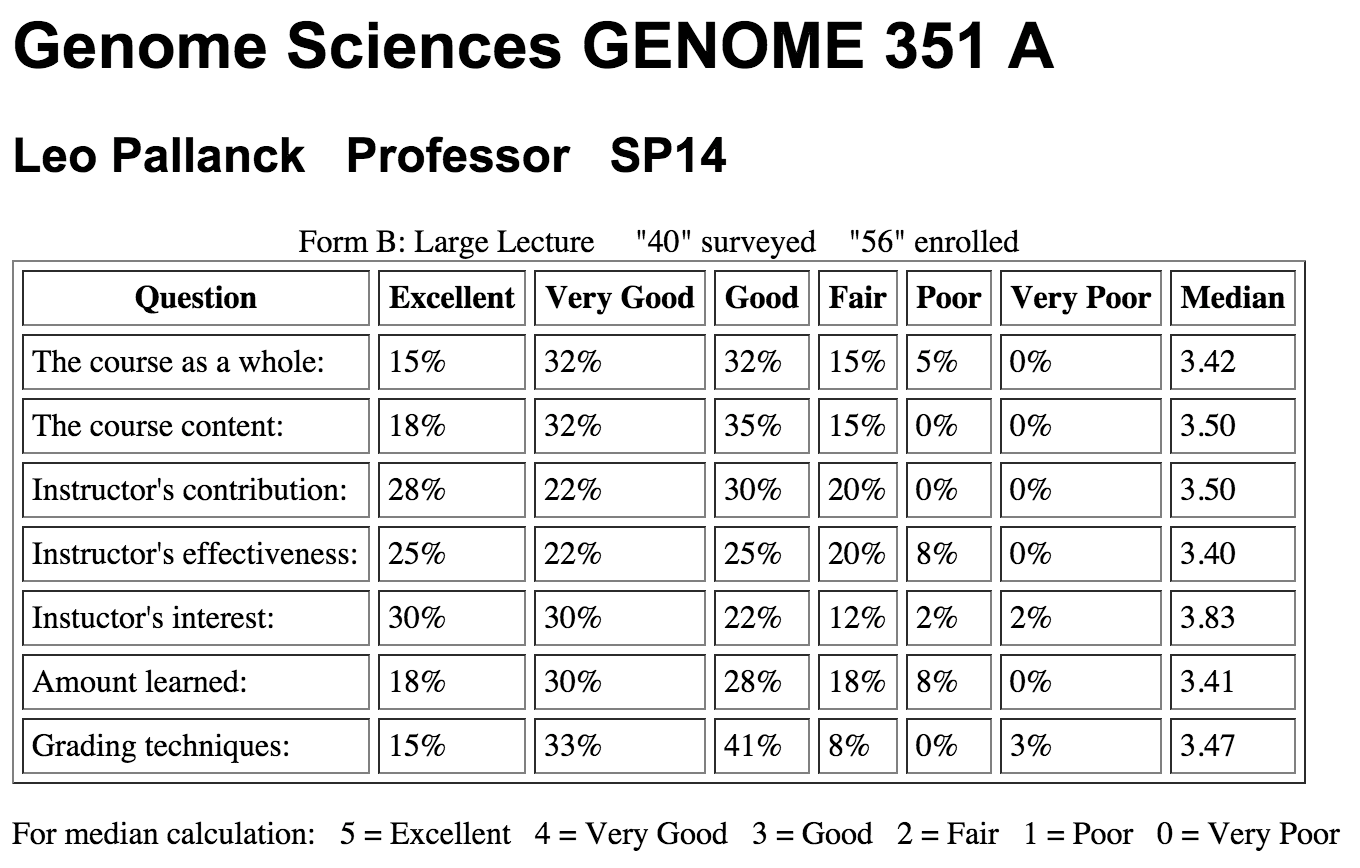
\includegraphics[width=0.4\textwidth]{cec_2.png}
\end{tabular}
\end{center}

The Course Evaluation Catalog is the main source for students at the University of Washington to check the reviews / ratings of a specific course that is offered at the University. At the end of each class, instructors are required to prompt a survey (either on-line in recent quarters or in class) that evaluates the instructor and the class on a number of different dimensions. This data is then posted on-line at some later date for the general public of the University to see. Unfortunately, only the past 2-3 quarters are kept on the site and the web application, if you could call it that, is incredibly difficult to use. Each entry is its own web page which contains a table displaying the information. The data that we use is scraped from this site (for the past 2 years).

\subsubsection*{RateMyProfessors (RMP) \cite{ratemyprofessors}}
{\color{blue} \href{http://www.ratemyprofessors.com/}{http://www.ratemyprofessors.com/}}

\vspace{-7 pt}
\begin{center}
\begin{tabular}{ll}
    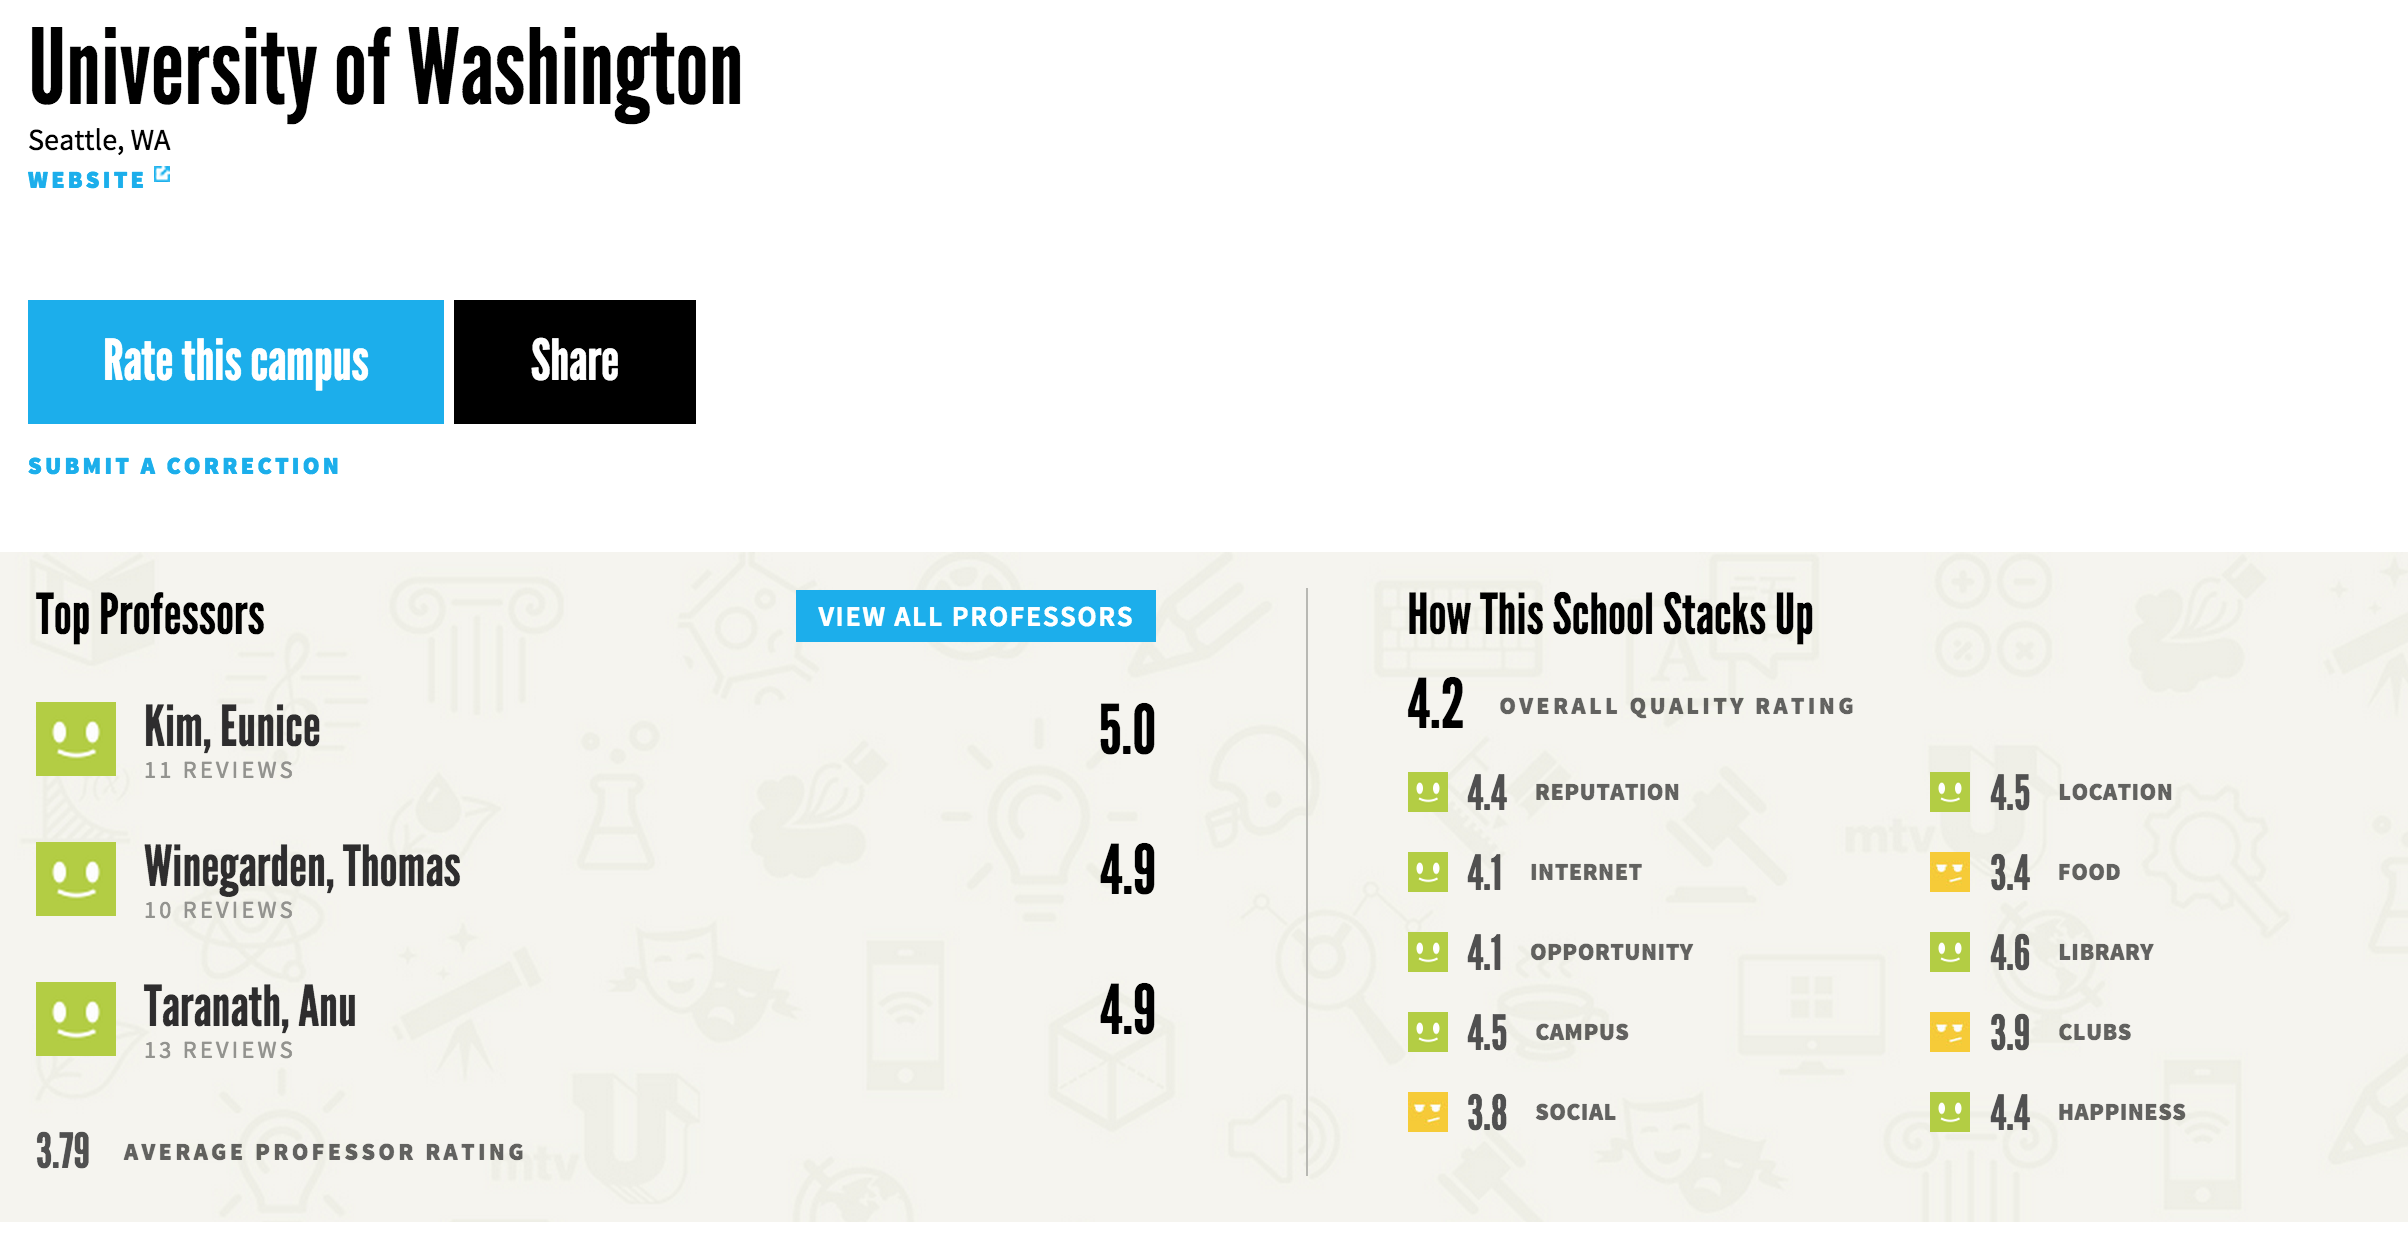
\includegraphics[width=0.62\textwidth]{rmp.png}
    &
    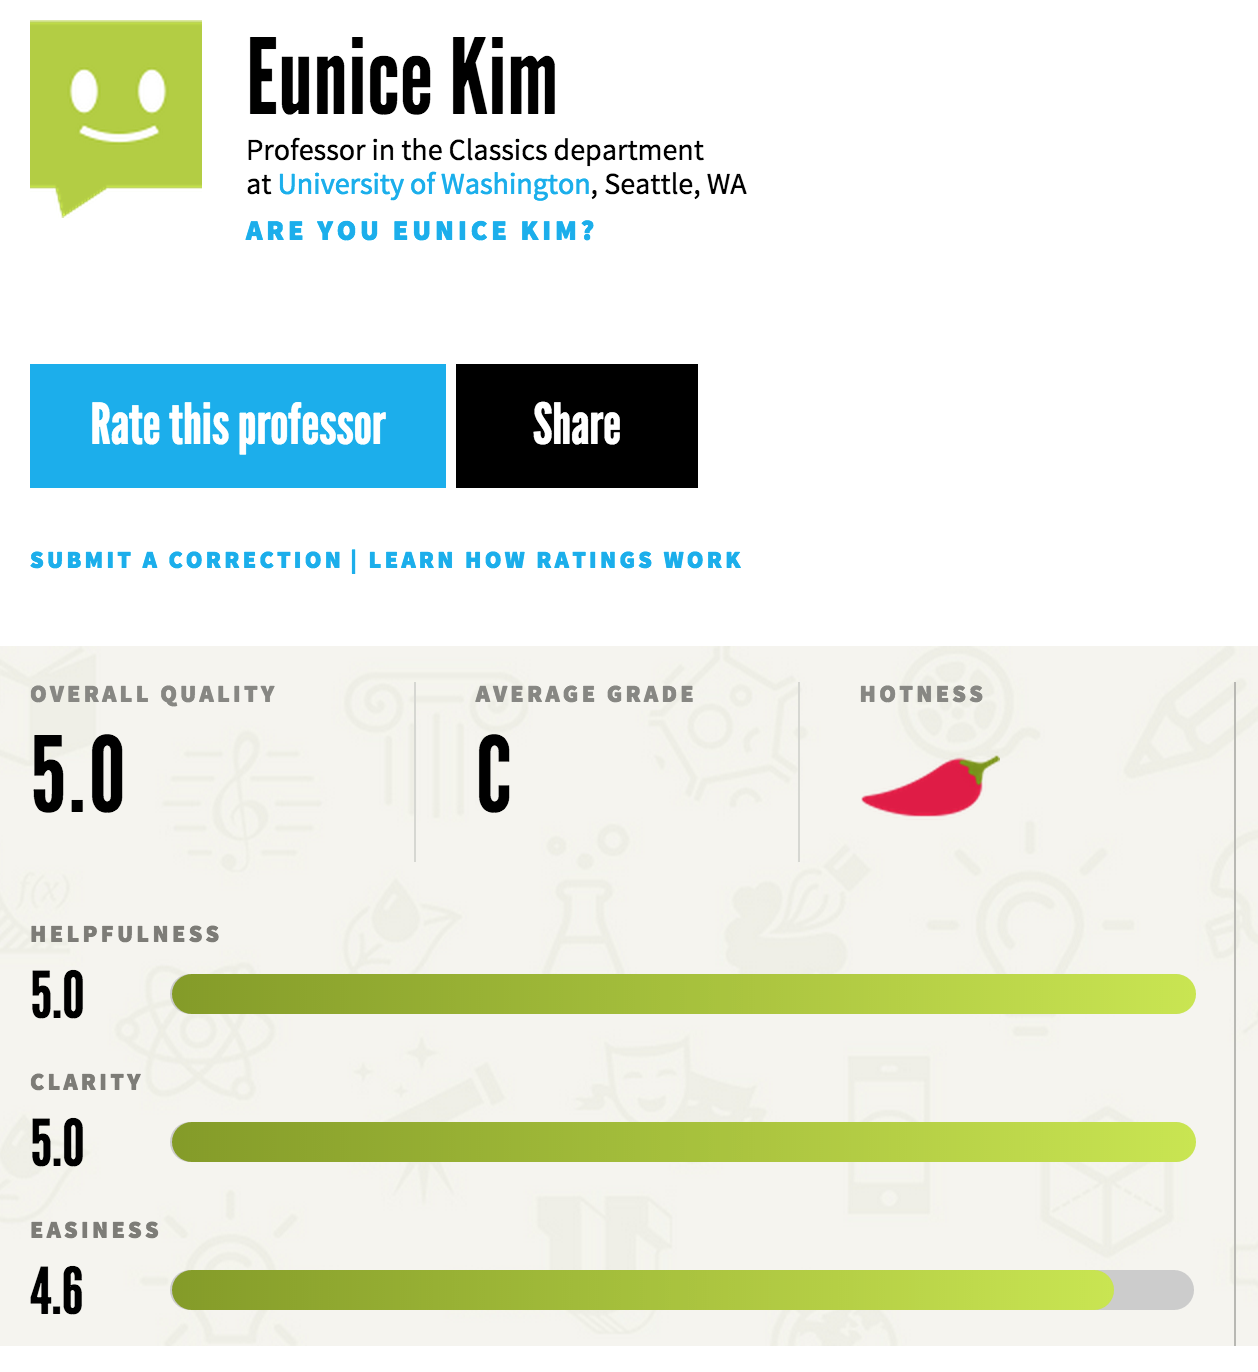
\includegraphics[width=0.33\textwidth]{rmp_2.png}
\end{tabular}
\end{center}

RMP was a tool created a while ago to encourage students to rate their teachers and professors since most Universities did not have publicly accessible data on the matter. It became quite popular and is still widely used today. RMP has been extensively criticized for having a poor representation of instructors and the student body that is doing the rating \cite{coladarci2007ratemyprofessors,felton2008attractiveness,sonntag2009empirical}. This is largely because the students that take the time to rate a specific instructor tend to have had a good or bad experience with him or her. This drives the aggregate rating towards the extremes. Another problem is that there tends to be a lack of data ($<$ 10 entries) for most instructors at most universities (including the University of Washington). This means there is not enough data to reliably make a decision since there aren't enough entries for a instructor for the ``wisdom of crowds'' effect to take place.

\subsubsection*{berkeleytime (BT) \cite{berkeleytime}}
{\color{blue} \href{http://www.berkeleytime.com/}{http://www.berkeleytime.com/}}

\vspace{-3 pt}
\begin{center}
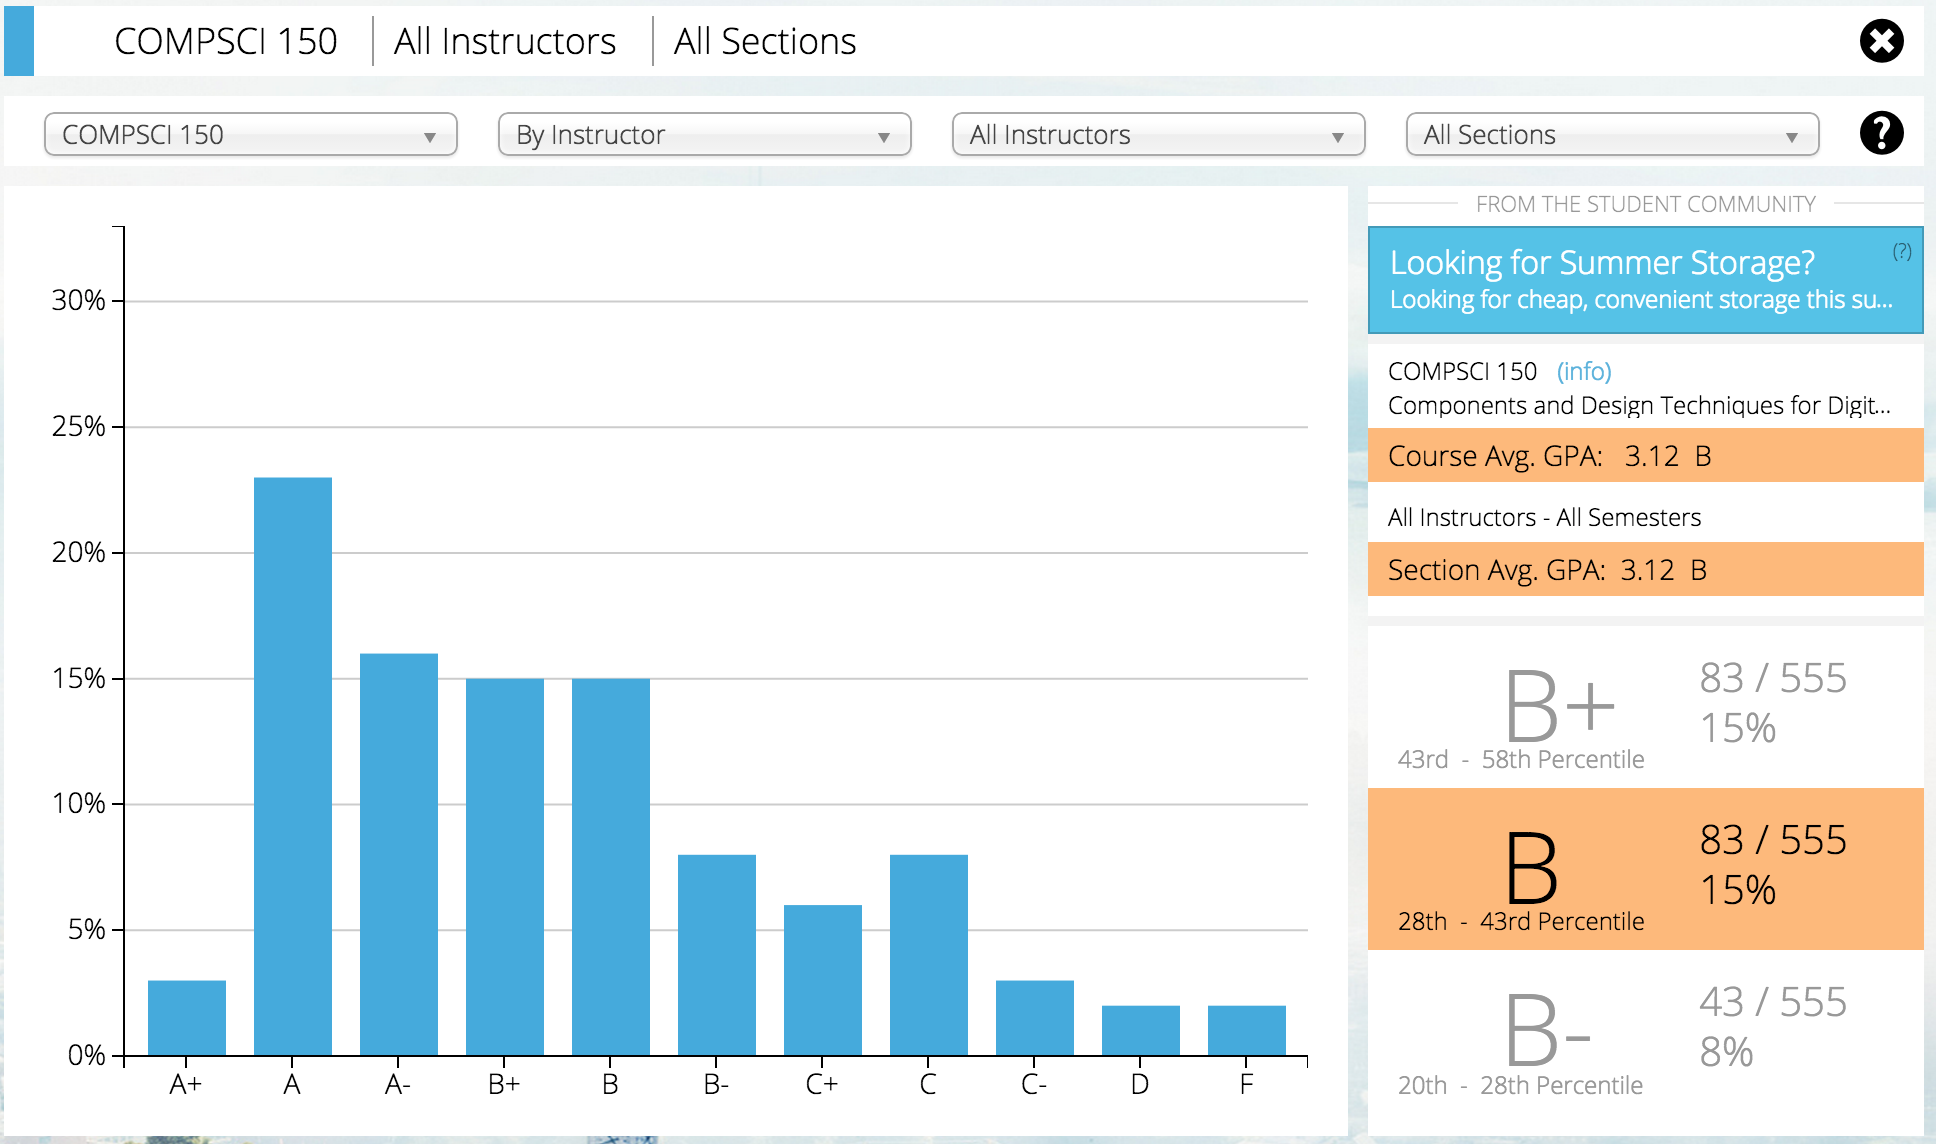
\includegraphics[width=0.7\textwidth]{bt.png}
\end{center}

BT was brought to our attention after explaining this project to fellow colleagues that happen to be in Berkeley's Computer Science Department. 3 undergraduates were able to convince the school to allow them access to the entire schools catalog of courses, which also happens to include the grade distributions of every class. This is the main use of the tool. Students can search for classes and directly see the grades that everyone received and then they can break it down by the instructor that taught the class. Unfortunately, the University of Washington does not provide this kind of data and it is highly unlikely that they ever would. Because of this, CourseRatings relies on the ratings of the class and not the grade distribution (although it could be said that these two quantities could be correlated).

\section*{Final Project Plan}

\begin{description}
    \item[5/21] Final Project Progress Presentation
    \begin{itemize}
        \item Receive feedback from peers on what can be improved or added in the design.
    \end{itemize}

    \item[5/25] Increase Quality and Amount of Data
    \begin{itemize}
        \item Update web scraping scripts (which broke on the CEC's latest update) to get the most recent quarter's data.
        \item Write a scraper for the course catalog to get the most up to date names of all the classes as well as their descriptions.
        \item Add a column in the results that indicates the percentage of students who filled out the survey.
        \item Add a description to each course's page that includes the newly scraped description.
    \end{itemize}

    \item[6/3] Implement New Features
    \begin{itemize}
        \item Collapse identical courses: entries with the same course number will be collapsed into a single entity, which will display the average of each entry within it. An arrow or button of some kind will indicate that this row can be clicked to expand all of the records of the course.
        \item Search redesign: Three separate drop-down boxes, each with the ability to search, will be used for Department / Course Code / Instructor. In addition to this, each search box will support auto-complete, which will filter the selections possible in the drop-down box by what is currently typed in its search field. Lastly, the drop-down box will only display options that are in agreement with the other 2 search boxes.
        \item Department visualization: if only a department is selected, create a visualization that shows general information about that specific department (for example: average overall rating, average grade, etc.).
    \end{itemize}

    \item[6/6] Small Modifications
    \begin{itemize}
        \item Reevaluate what we have created and make any small improvements / corrections.
        \item Present to friends and colleagues for feedback to be used in the final writeup.
    \end{itemize}

    \item[6/8] Final Poster Presentation
    \begin{itemize}
        \item Working demo of what we created.
        \item Final poster depicting the thought we put in to the problem we solved and the project.
    \end{itemize}

    \item[6/11] Final Deliverables
    \begin{itemize}
        \item PDF of poster we created for the poster presentation.
        \item Finished paper about our project.
        \item Final code.
    \end{itemize}
\end{description}

\bibliographystyle{apalike}
\bibliography{sources}

\end{document}
